\chapter{NES FPGA alapú újragondolása}

A diplomaterv projektem egyik fő célja, hogy egy hardveres emulátort készítsek a Nintendo Entertainment System játékkonzolhoz. Alapvetően emulátort lehet készíteni szoftveres, illetve hardveres módon. A szoftveres emulátorok alapja az eredeti hardver szimulálása egy magasabb programozási nyelven íródott szoftver segítségével (pyton, java). Viszont ezek az emulátorok az esetek többségében nem tudják az eredeti hardver időzítésit pontosan betartani, ezért nem teljesen autentikus a játék élmény. Hardveres emulálásnál általában egy FPGA chipet használnak és ebben implementálják az eredeti hardveres működéseket. Az általunk választott megvalósítás sokkal időigényesebb, viszont ennek segítségével képesek vagyunk az eredeti eszköz pontosabb emulálására. Illetve egy erősebb FPGA segítségével modernizálhatunk egy régebbi konzolt is, persze bármilyen hardveres módosítás esetén (amely eltér az eredeti eszköztől) át kell gondolnunk, hogy a megváltozott körülmények között is képesek leszünk-e futtatni az eredeti szoftvereket a hardveren. 

Ebben a fejezetben azt fogom bemutatni, hogy milyen hardveres változtatásokat/fejlesztéseket eszközöltem, az eredeti NES-hez képest, hogy egy friss, modernebb megjelenést adjak az eredeti konzolnak.

\section{Képalkotás}
\label{sec:picture-creation-ideas}

Már az előző \ref{subsec:PPU-CRT}. fejezetben olvashattuk, hogy a NES egy kompozit jelet állított elő CRT televíziók számára. Ez talán a játékkonzol legelavultabb része, hiszen napjainkban már ezt a televízió típust nem is lehet beszerezni. Ezeket teljes mértékben leváltották a VGA alapú (DVI, HDMI, DisplayPort csatlakozóval ellátott) különböző méretű és felbontású lapos TV-k. Ezeknek a megvalósításoknak rengeteg előnye van az analóg megjelenítéssel szemben. Az egyik legjelentősebb, hogy ezen keresztül képesek vagyunk a torzításmentes átvitelre.

A NES eredeti felbontása 256x240 pixel és 60 Hz (NTSC). Ez a  méret sajnos nem felel meg a modern VGA szabványoknak, úgyhogy ezen a téren módosítanunk kell a PPU képgenerálásán. A módosítások során a VGA adatok generálását helyeztem előtérbe. A legkisebb VGA kép méret, amivel érdemes dolgozni és a modern TV-k és monitorok is támogatják, az a 640x480 pixel és 60 Hz. Ebben a méretben pontosan elfér a kétszeres NES képméret. Tehát, ha egy NES pixelt 2x2 pixellel reprezentálunk, akkor 512x480 pixel méretű képet kapunk. Ennél bonyolultabb megoldás is létezik (bilineáris interpoláció), de a sima nagyítás a legegyszerűbb, ezért kezdetben ezt implementálom. Ez a változtatás lehetővé teszi, hogy NES nyomtatott huzalozott kártyáján modern HDMI csatlakozót helyezzek el. 

Illetve ebből a módosításból következőleg a rendszerünk működési frekvenciája is megváltozik, a VGA jelünk pixel órajele 25 MHz lesz, az TMDS adatok pedig 250 MHz-el lesznek továbbítva a TV vagy monitor felé. Ez azt jelenti, hogy a PPU-nk működési órajelét is meg kell változtatni. Ez eredetileg körülbelül 5.37 MHz az NTSC modellben. A NES nyomtatott huzalozott kártyáján, ezért egy magasabb frekvenciájú órajel forrást kell elhelyezni. Az órajel pontos beállítására pedig az FPGA chip DCM (Digital Clock Manager) és PLL (Phase Locked Loop) funkcióit használhatjuk.  

\section{Audio}
%todo fűzd össze a audio bemutatásával
Az audió feldolgozó egység (Audio Process Unit, APU), egy öt különálló hangsávot kezelő analóg komponens, mely a NES eredeti hangját nem lineáris keverés segítségével állította elő. Ezt a jelet a hardveres emulálás során mi egy digitális jelként állítjuk elő az FPGA-val. Ahhoz, hogy az eredeti eszköz hangját élvezni tudjuk, ezt először egy DAC segítségével analóg jellé kell konvertálnunk, végül pedig egy megfelelő erősítőn át egy Jack csatlakozóra kivezetnünk. Az erősítő típusa attól függ, hogy fülhallgatón vagy pedig hangszórón szeretnénk, hogy ezek az ikonikus dallamok megszólaljanak. Jó kompromisszumos megoldás lehet a kártyát fülhallgató erősítővel ellátni, mivel a hangszórókból léteznek olyan modellek (belső erősítővel rendelkezők), amelyek ezzel a gyengébb erősítővel is működnek, így mind a két opció fennáll a konzol használatára. Az eredeti konzol mono hangzással rendelkezett, viszont mi ezt jelet a DAC működése miatt, mind a két fülre kivezethetjük, ezzel sztereó hangzást imitálva (ettől még természetesen ez nem lesz valódi sztereó jel).   

Mivel a NES nyomtatott huzalozott kártyáján már a képalkotás miatt elhelyezek egy HDMI csatlakozót, ezért ennek a videó csatornáin át tudom küldeni a verikális visszafutás ideje alatt az adudió adatokat is. Viszont ehhez szükségem van egy I2C interfészre ahhoz, hogy a megjelenítő EDID ROM-ját ki tudjam olvasni, amelyből megállapítható, hogy képes-e audió adatok vételére az eszköz. Így lehetővé téve, hogy egy esetleges későbbi fejlesztés során a TV vagy monitor beépített hangszóróján szólaljon meg játékkonzolunk. 

\section{Játékok tárolása}
\label{sec:Game-store}
%todo fűzd össze a kazetták bemutatásával
A NES játékok programkódja és Pattern tábla adatai az esetek többségében a játékkazetta saját program és karakter ROM-jában helyezkedtek el. A játékkártyák befogadása rengeteg extra területet emésztene fel a nyomtatott huzalozott kártyán, mert a kazetta befogadó egységet rá kellene tervezni az eszközre, illetve az összes teszt játéknak fizikailag a birtokomba kell lennie ehhez, ebből adódóan az egyéb hardveres teszteket is nehezen lehetne megvalósítani. 

Ennek következtében egy új megoldást kell kitalálni arra, hogy az emulált NES hardvert megfelelő módon ellássam a játékokkal. Az egyik kézen fekvő megoldás, hogy a hordozó kártyára el lehet helyezni egy statikus RAM modult, amelynek elég nagynak kell lennie ahhoz, hogy a játék kártyák karakter és program ROM-ját egyszerre tartalmazza. A legnagyobb NES játék 768 KB memória területtel rendelkezik (Kirby's Adventure), ehhez képest az összes többi játék 512 KB-os vagy ennél kisebb méretű. A NES hardvernek indítás előtt ezt a SRAM-ot fel kell töltenie a játékkal, majd a konzol indítását követően a PPU és CPU innen fog dolgozni.

Annak érdekében, hogy több játékot is képesek legyünk tárolni, érdemes egy nagyobb méretű háttértárat is tervezni az eszközre, amely a játékokat fogja tartalmazni. Erre ideális lehet egy SD kártya. A projekt kezdeti szakaszában ezt még nem használom, viszont az esetleges jövőbeli fejlesztések miatt érdemes, már most a kártyára tervezni egy ilyen olvasót.

A NES hardver belső memória területeit, pedig az FPGA-ban kialakítható Blokk/LUT RAM-okban helyezhetjük el (Névtáblák, OAM, másodlagos OAM).

\section{Kompakt hordozható méret}
\label{sec:Size}

A NES újra tervezésének egyik fő aspektusa a méret csökkentése. Az eredeti konzol 256 mm hosszú, 203,2 mm széles és 88,9 mm vastag volt. Ez a modern nyomtatott áramkörök tervezésével és a komponensek méretével sokkal kisebb területre csökkenthető. Ezzel kompakt hordozható kialakítást kölcsönözve a játékkonzolnak.

%todo fekete fehét kép
\begin{figure}[H]
	\centering
	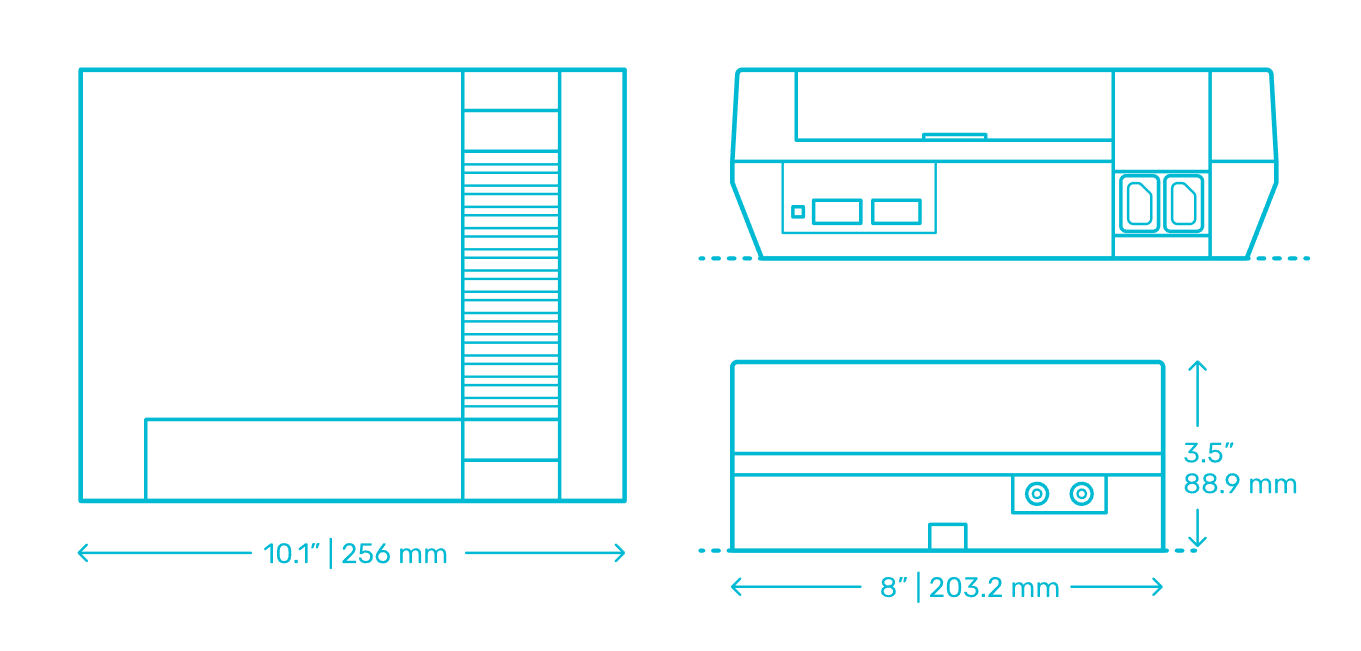
\includegraphics[width=150mm, keepaspectratio]{figures/NES-size}
	\caption{A NES játékkonzol dimenziói \cite{NES_dimensions}}
	\label{fig:NES-size}
\end{figure}

A kompakt méret mellett szerettem volna megőrizni az eszköz nosztalgia faktorát is, ezért a kártyámon elhelyeztem két eredeti NES játék kontroller csatlakozót (kooperatív játékok miatt). Ez természetesen az eredeti hardver kontrollereivel kompatibilis.


